\documentclass[dvisvgm,tikz]{standalone}
\begin{document}
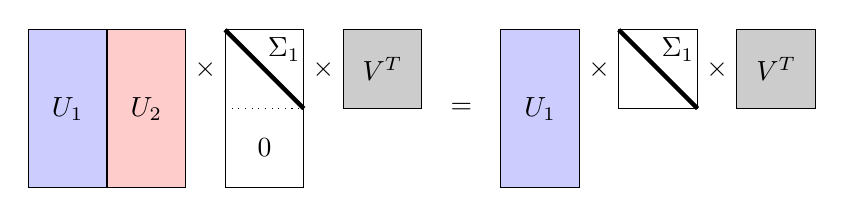
\begin{tikzpicture}

  % Full factorization
  \begin{scope}[shift={(0,0)}]
  \filldraw[fill=blue!20] (0,0) rectangle (1,2);
  \filldraw[fill=red!20] (1,0) rectangle (2,2);
  \draw (2.5,0) rectangle (3.5,2);
  \draw[dotted] (2.5,1) -- (3.5,1);
  \draw[ultra thick] (3.5,1) -- (2.5,2);
  \filldraw[fill=black!20] (4,1) rectangle (5,2);
  \node at (0.5,1) {$U_1$};
  \node at (1.5,1) {$U_2$};
  \node at (3.25,1.75) {$\Sigma_1$};
  \node at (3,0.5) {$0$};
  \node at (2.25,1.5) {$\times$};
  \node at (3.75,1.5) {$\times$};
  \node at (4.5,1.5) {$V^T$};
  \end{scope}

  % Economy factorization
  \begin{scope}[shift={(6,0)}]
  \filldraw[fill=blue!20] (0,0) rectangle (1,2);
  \draw (1.5,1) rectangle (2.5,2);
  \draw[ultra thick] (1.5,2) -- (2.5,1);
  \filldraw[fill=black!20] (3,1) rectangle (4,2);
  \node at (0.5,1) {$U_1$};
  \node at (2.25,1.75) {$\Sigma_1$};
  \node at (1.25,1.5) {$\times$};
  \node at (2.75,1.5) {$\times$};
  \node at (3.5,1.5) {$V^T$};
  \end{scope}

  \node at (5.5,1) {$=$};
\end{tikzpicture}
\end{document}
